\section{Ciência por trás dos dados}
Como um ser humano, os dados têm seu ciclo de vida, esse ciclo pode alterar-se dependendo de sua finalidade dentro da aplicação. O tema e o objetivo desta pesquisa é coberto por uma matéria, já antiga, nomeada KDD ou \textit{Knowledge Discovery in Database}, como o próprio nome traduzido sugere, a Descoberta de Conhecimento em Base de Dados abrange varias subclasses como mineração de dados, análise de dados, probabilidade e até mesmo a própria IA. A KDD se justifica pela sua metodologia de manipulação de dados afim de extrair o conhecimento almejado de um base. Ao observar o fluxo descrito na Figura \ref{fig:kdd}, pode-se notar que uma cadeia de eventos como: seleção, pré-processamento, mutação, mineração e interpretação. Esses eventos geram novos estados para o dado, e os moldam focando o objetivo de retirar o conhecimento pela interpretação no final do processo.

\begin{figure}
    \centering
    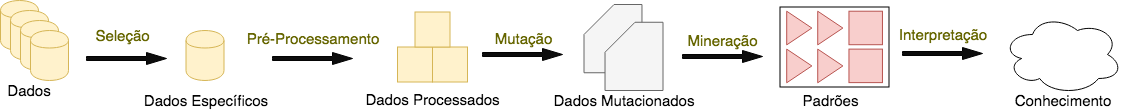
\includegraphics[width=.8\textwidth]{imagens/kdd.png}
    \caption{Representação da metodologia defendida pela KDD. Fonte: o autor.}
    \label{fig:kdd}
\end{figure}

Com o passar do tempo, várias abordagens surgiram para tratar dados e essa massa de pesquisas e definições deu-se por bagunçar em partes as nomenclaturas e definições que estão atrelados a ciência por trás dos dados. Para evitar confusões as definições apresentadas nessa sessão serão sucintas e tem como objetivo futuros tópicos e discussões apresentados durante os resultados dessa pesquisa. Devido a grande divergência, ocorrida pela disseminação rápida de algumas termologias, os termos abordados serão guiados pelas seguintes referencias \cite{laender2002brief, fayyad1996kdd, hand2007principles}.

\subsection{Coleta de Dados}
A coleta, é o ato de obter dados em massa de fontes externas, como \textit{websites} e \textit{apis}\footnote{A sigla API vem de \textit{Application Programming Interface} e é uma interface que permite outras aplicações utilizarem de seus recursos e funcionalidades. Dentro do universo \textit{web}, o termo API é utilizado para descrever um conjunto de rotas que podem ser utilizados para acessar recursos de um aplicação online.}. Também conhecido como \textit{data collection}, durante o processo do KDD é o primeiro passo responsável por gerar um amostra mais focada no problema.

No projeto será utilizada a API do Twitter para coletadar os dados para uso da aplicação. Durante a coleta é necessário entender as limitações da fonte de dados. No caso das API's é usual existir \textit{Rate Limits}, ou seja, limites de requisições, no caso do Twitter existem planos que aumentam ou diminuem seu acesso a API, no caso do projeto será utilizado a versão \textit{Standard} que é a versão gratuita para desenvolvedores\footnote{\url{https://developer.twitter.com/en/docs/basics/rate-limits.html}}. Alguns dos \textit{endpoints}\footnote{Um endpoint é uma URL acessivel por protocolos HTTP ou HTTPS e que retornam dados ou realizam ações} que serão:
\begin{itemize}
    \item \textit{users/show}: Responsável por pegar as informações do usuário, tem um limite de 60 requisições por minuto.
    \item \textit{statuses/user\_timeline}: Responsável por pegar os últimos tweets do usuário, tem um limite de 100 requisições por minuto.
\end{itemize}

Existe no projeto também, e recorrente em outros tipos de APIs, os \textit{streamings}, ou seja, recursos que serão consumidos através de uma requisição que fica aberta por tempo indeterminado recebendo novos dados.
\begin{itemize}
    \item \textit{statuses/filter}: Responsável por pegar os últimos tweets publicados por filtros. Na documentação será detalhado os filtros que serão utilizados na pesquisa, mas basicamente aqui é possível escutar as ultimas publicações feitas em escala global e coletar apenas as que compatíveis com um conjunto de filtros. Esse tipo de recurso não tem seu limite estabelecido por requisições e sim pelo seu uso (tentativas de reconexões por exemplo).
\end{itemize}

Uma vez coletados, outras ações descritas na Figura \ref{fig:kdd} como Pré-Processamento e Mutação serão realizados no próprio coletor enquanto outras serão realizadas posteriormente por \textit{scripts} e/ou ferramentas. A preparação do dado é relevante para assegurar a qualidade da mineração. No Twitter pode-se encontrar diversos problemas na hora da análise. Alguns dos mais populares são: A quantidade de ruído apresentado nos dados por erros de ortográfica, os uso de símbolos especiais como \textit{emojis} ou a inserção \textit{urls} ao longo do texto e por final a informalidade e contexto multilíngue, ou seja, o ato de escrever-se utilizando palavras fora do nosso idioma ou gírias pra manifestar algo. Além disso existe o fato de alguns processamentos, como a análise de sentimento, ter alguns problemas em textos muito curtos ou muito compridos. Pesquisas de 2012\footnote{\url{https://thenextweb.com/twitter/2012/01/07/interesting-fact-most-tweets-posted-are-approximately-30-characters-long/}}, demonstram que um tweet contém em média apenas 30 caracteres com o seu limite máximo, já pequeno, de 140 carácteres. \cite[9-11]{silva2016analise} Entretanto, no dia 27 de setembro de 2017, o Twitter anunciou\footnote{\url{https://blog.twitter.com/official/en_us/topics/product/2017/Giving-you-more-characters-to-express-yourself.html}} a expansão do limite máximo para 280 caracteres, o que abre possibilidade de textos mais pontuais na massa de dados coletada.

Uma vez conhecida as limitações e problemas da fonte de coleta, é possível idealizar e implementar soluções para contornar e/ou utilizar alguns recursos apresentados problemáticos.

\subsection{Mineração de Dados}
A mineração é um passo que ocorre após os dados terem sido devidamente normalizados. Vale ressaltar que para obter conhecimento não é necessário uma IA, sistemas de tomada de decisão trabalham com probabilidade matemática sob dados exatos, o que em muitos casos, já seria o suficiente para obter a informação do dado. Entretanto, o foco da pesquisa se baseia na implementação de um sistema inteligente e isso inclina essa explicação para o fato de: o aprendizado de máquina é uma das possíveis formas de se minerar um dado.

A mineração de dados ou popularmente conhecida como \textit{data mining}, baseia-se em retirar os valores mais relevantes e valiosos para se inferir um conhecimento. Os demais passos como pré-processamento e mutação se assemelham a alguns processos citados anteriormente como a redução dimensional ou ainda a engenharia de atributos.

No caso dessa pesquisa, a inferência de uma EADS baseada nas publicações de um usuário seria um tipo de dado extraído a partir de um modelo inteligente treinado por uma base de dados pré-processada. A caracterização de um perfil baseado em seus atributos, incluindo o próprio valor da EADS inferido, seria um outro exemplo do uso de IA para minerar a probabilidade de existir um certo nível de uma ou mais dimensão afetiva baseada em informações pessoais como sexo, localidade, trabalho e gostos pessoais.

Existem pesquisas voltadas a identificação de depressão dentro do Twitter, alguns dos atributos estabelecidos por eles como frequencia de postagem, a hora de maior atividade na rede social, sua interação com demais usuarios e até o óbvio uso de nome de antedepressivos nas frases, são taxados como ótimos atributos durante a mineração. \cite{de2013social, de2013predicting, tsugawa2015recognizing, yang2015gis}.

Com os dados em mãos, é possível, baseado no conhecimento fornecido pelo dado, realizar vários tipos de análise. O enfoque desse trabalho não é realizar hipóteses ou explorar os dados gerados, e sim, certificar a possibilidade da criação dessa base e a assertividade dos modelos, garantindo, que outros pesquisadores possam utilizar da base gerada nesse trabalho para realizar futuras pesquisas. Mesmo assim se torna relevante citar, mesmo que brevemente, a última parte do ciclo de um dado referente a consumir o conhecimento fornecido pelo mesmo.

\subsection{Análise de Dados}
O passo descrito como interpretação no KDD se refere a entender os dados de saída vindos da mineração afim de afirmar ou descartar hipóteses, com isso é possível refinar o processo e/ou explorar novas possibilidades. Existem 3 fortes termos quando tratamos a analise de dados:
\begin{itemize}
    \item - \textit{Data Exploration}: O ato de explorar os dados (conhecimento) gerados afim de localizar pontos relevantes e elaborar ou embasar hipóteses.
    \item - \textit{Data Storytelling}: O ato do dado contar uma história. Abordar a hipótese de maneira empírica e demonstrar a veracidade dela discutindo abordagem e algoritmos gerados é um dos objetivos dessa área.
    \item - \textit{Data Visualization}: O ato de demonstrar o dado através de representações gráficas ou tabelas, normalmente utilizados para embasar e demonstrar dados durante o \textit{Storytelling}.
\end{itemize}

Todos os conceitos apresentados acima, utilizados em conjunto ou separado, são parte necessária do processo de IA. Durante a pesquisa serão utilizados tais recursos com a premissa de refinar nosso processo de mineração/aprendizado, como demonstrar alguns dados gerados pela pesquisa.
